%!TEX root = main.tex
\documentclass[main.tex]{subfiles}

\begin{document}

\section{Basic Functionality}
As a reminder, the various small goals were listed in Section \ref{sec:test-basic}. They are listed here again for clarify. These were little goals that were achieved throughout the implementation. The results for each item is found in Table \ref{tbl:basic-goals}.

\begin{enumerate}
	\item RasPBX installed, internal network functioning
	\item Obi110 configured with RasPBX, calls passing through
	\item Calls directed to an IVR for naive filtering
	\item Switch working correctly
	\item Audio detected and extracted
	\item Speech-to-text and call metric working
	\item Display system working (server and webpage)
	\item Both call analysis functions and server function working together
	\item Bypass switch
\end{enumerate}

The only unsuccessful mini-goal is the bypass switch that was discussed in the Design section. This was primarily due to the time constraints of the project. The voice recognition and voice prompt interaction were given a higher priority over this feature, which is a safety fallback. The reasons for this, and the impact of this on the functionality are included the Evaluation section.

\begin{table}[htb]
\centering
\begin{tabular}{|l|l|}
	\hline
\textbf{Item Number} & \textbf{Successful?}                                 \\\hline
1           & Yes                                                    \\
2           & Yes                                                   \\
3           & Yes                                                 \\
4           & Yes                                                 \\
5           & Yes                                                 \\
6           & Yes                                                \\
7           & Yes                                                \\
8           & Yes                                                \\
9           & No  \\\hline
\end{tabular}
\caption{Success of the various goals. }
\label{tbl:basic-goals}
\end{table}

\section{Robustness}
The results of the transcription tests are found in Table \ref{tbl:robust}. The various sentences that were used from Scam Call Fighters \cite{spam-calls}, along with the Youtube transcriptions were all passed through the metric, and the risk rating is shown. They various scam transcripts are referred to by a number, and their exact content is found in the repository as mentioned in Appendix \ref{sec:appendix-repo}.

\begin{table}[htb]
\centering
\begin{tabular}{|l|l|}
	\hline
\textbf{Scam Number} & \textbf{Risk Level}                                 \\\hline
1           & Medium                                                    \\
2           & Medium                                                   \\
3           & Medium                                                 \\
4           & Medium                                                 \\
5           & Medium                                                 \\
6           & Medium                                                \\
7           & Medium                                                \\
8           & Low                                                \\
9           & Medium                                                \\
10           & Medium                                                \\
11           & High                                                \\
12           & Low                                                \\
13           & Medium  \\\hline
\end{tabular}
\caption{Estimated risk levels of the various scam call transcripts. }
\label{tbl:robust}
\end{table}

\section{Ease of Caller and User Interface}
\subsection{Scores from the Questions}
A total of 15 people were involved in this small survey. The results of their scores are as shown in Table \ref{tbl:survey}, while the mean score is shown in Table \ref{tbl:mean}.

\begin{table}[htb]
\centering
\begin{tabular}{|c|ccccccccccccccc|}
	\hline
\textbf{Question} & \multicolumn{15}{|c|}{\textbf{Score}} \\\hline
\textbf{1} & 5 & 3.5 & 4 & 4 & 5 & 5 & 3 & 2.5 & 4 & 5 & 4 & 3 & 4 & 5 & 4 \\
\textbf{2} & 5 & 4 & 5 & 4 & 5 & 4 & 2.5 & 3 & 5 & 4 & 5 & 3 & 4 & 5 & 4 \\
\textbf{3} & 4 & 4 & 5 & 3 & 5 & 5 & 4 & 3.5 & 5 & 4 & 3 & 5 & 3 & 4 & 5 \\
\textbf{4} & 5 & 5 & 4 & 4 & 5 & 5 & 2 & 4 & 5 & 5 & 5 & 5 & 4 & 4 & 4 \\
\textbf{5} & 4 & 1 & 5 & 5 & 4 & 5 & 4 & 5 & 5 & 5 & 5 & 3 & 2 & 5 & 3 \\
\textbf{6} & 4 & 3.5 & 3 & 2 & 3 & 3 & 5 & 5 & 5 & 4 & 2 & 5 & 3 & 1 & 4\\\hline
\end{tabular}
\caption{User Interface and Ease of Caller survey results}
\label{tbl:survey}
\end{table}

\begin{table}[htb]
\centering
\begin{tabular}{|c|cccccc|}
	\hline
\textbf{Question} & 1 & 2 & 3 & 4 & 5 & 6\\\hline
\textbf{Mean} & 4.0667   & 4.1667   & 4.1667    &4.4000   & 4.0667   & 3.5000\\\hline
\end{tabular}
\caption{Mean score of each question.}
\label{tbl:mean}
\end{table}



\begin{figure}[htb]
	\captionsetup[subfigure]{position=b}
        \centering
        \begin{subfigure}{.47\textwidth}
                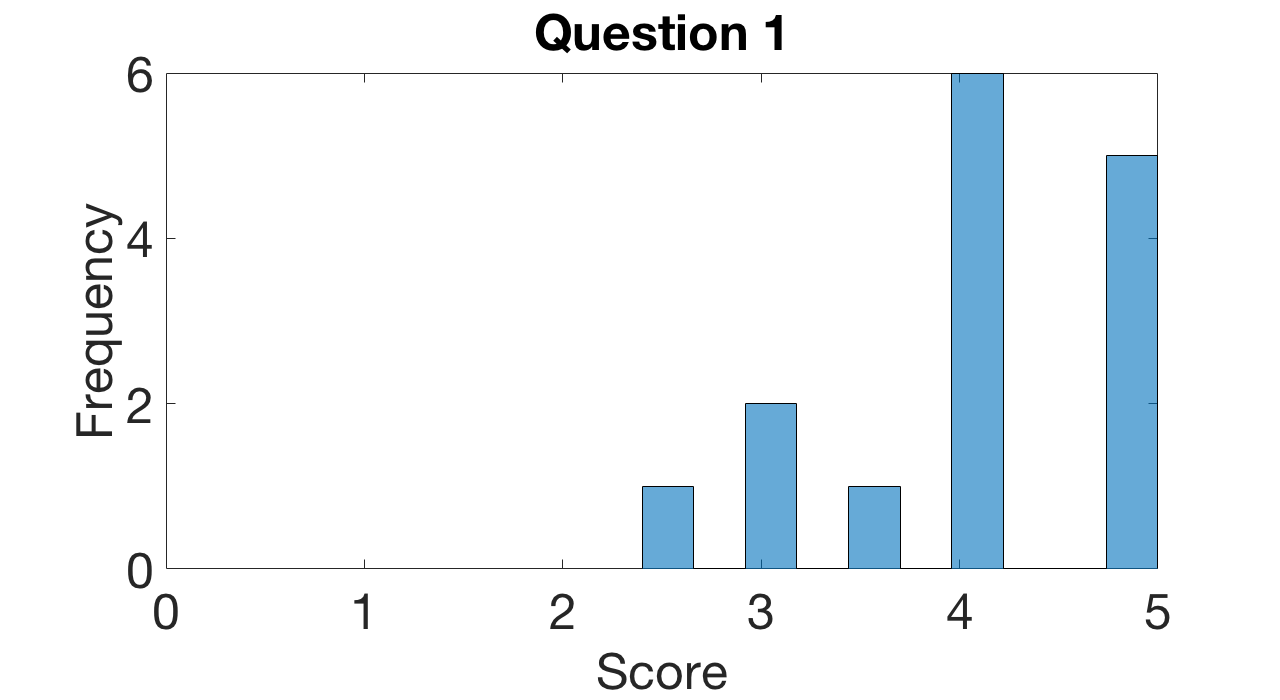
\includegraphics[width=\textwidth]{pics/q1}
                \caption{Question 1.}
                \label{fig:survey1}
        \end{subfigure}
        ~
		\begin{subfigure}{.47\textwidth}
                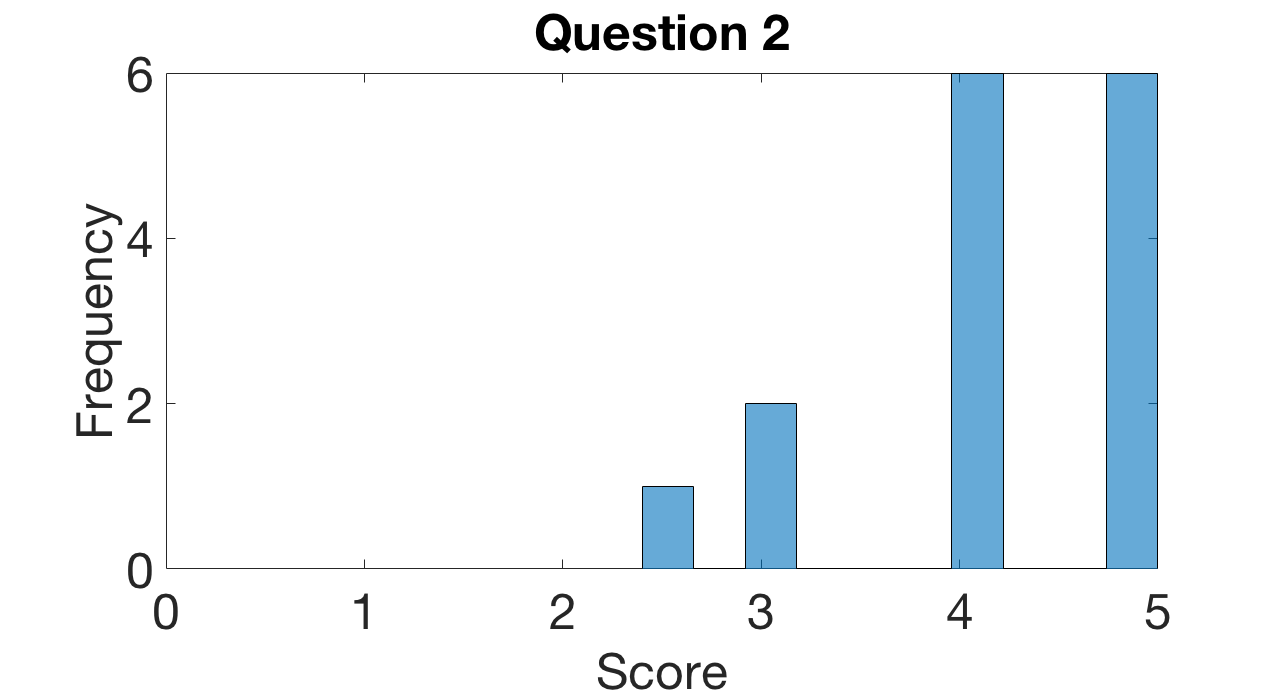
\includegraphics[width=\textwidth]{pics/q2}
                \caption{Question 2.}
                \label{fig:survey2}
        \end{subfigure}
		\\
		\begin{subfigure}{.47\textwidth}
				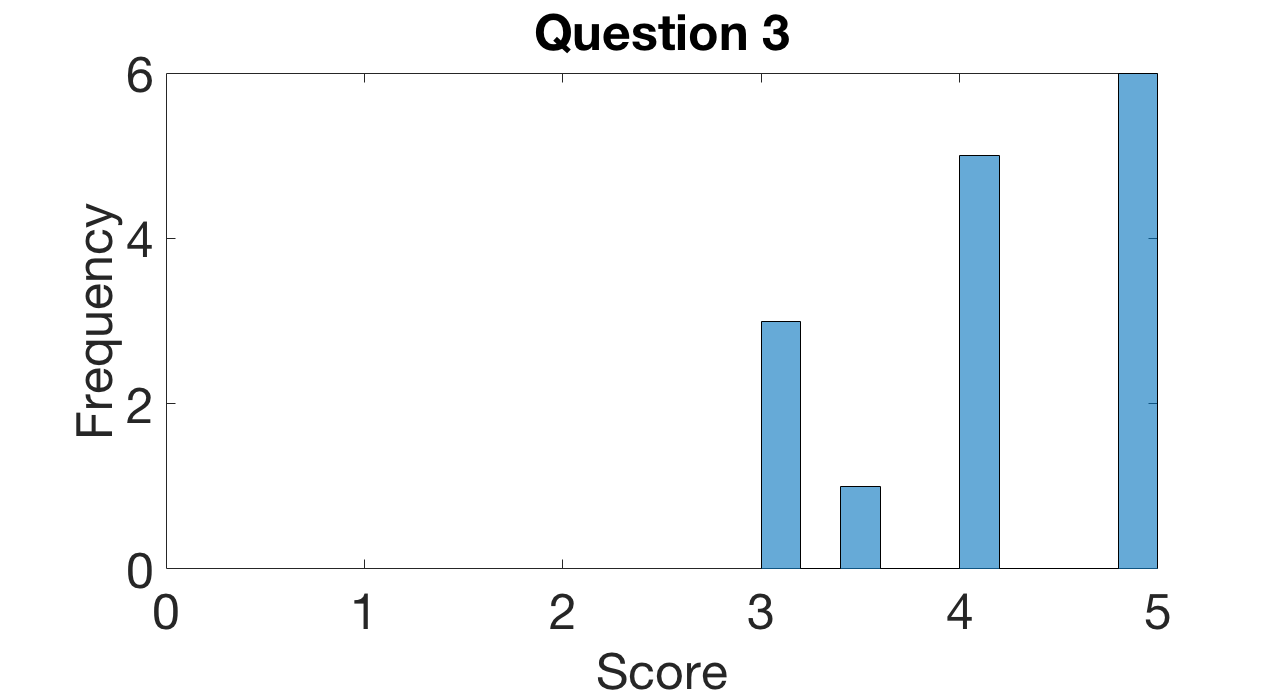
\includegraphics[width=\textwidth]{pics/q3}
				\caption{Question 3.}
				\label{fig:survey3}
		\end{subfigure}
		~
		\begin{subfigure}{.47\textwidth}
				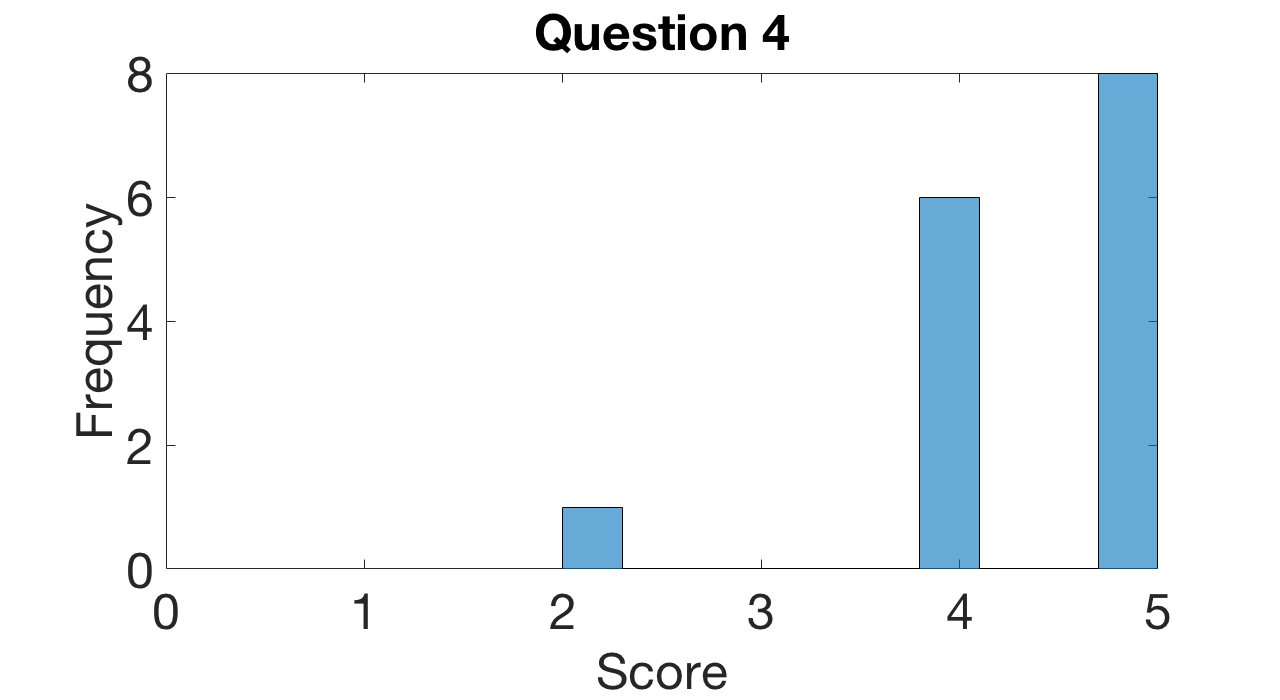
\includegraphics[width=\textwidth]{pics/q4}
				\caption{Question 4.}
				\label{fig:survey4}
		\end{subfigure}
		\\
		\begin{subfigure}{.47\textwidth}
				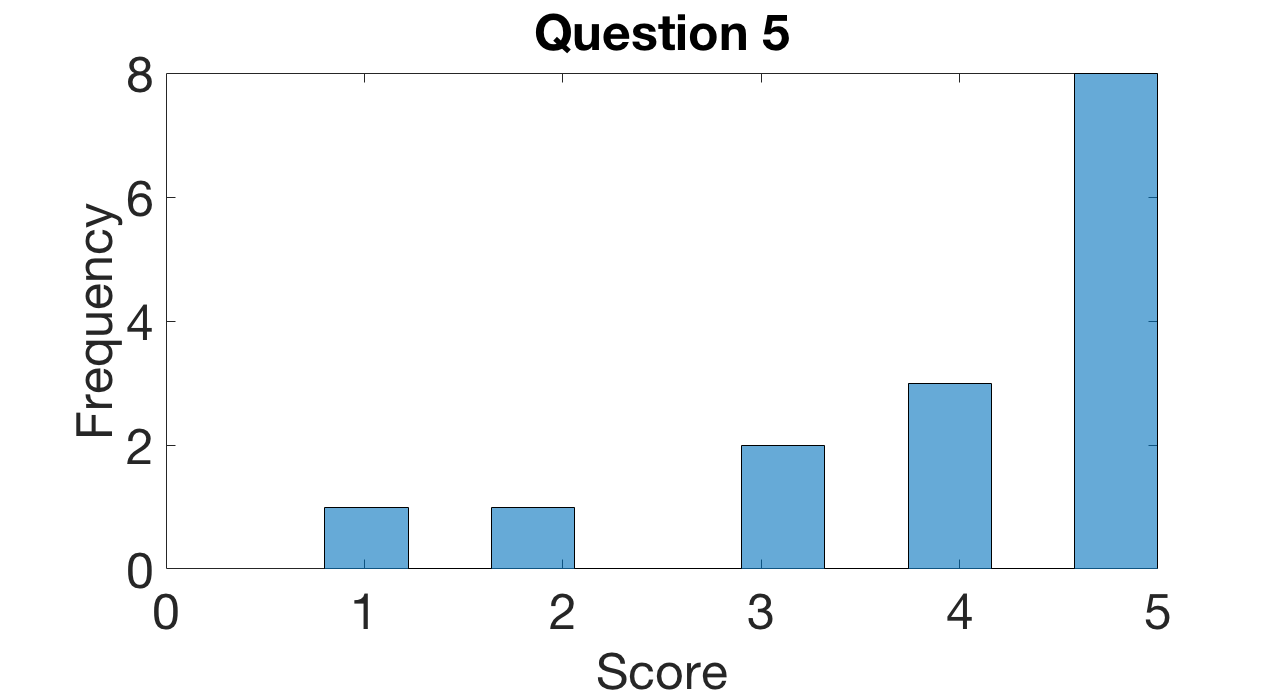
\includegraphics[width=\textwidth]{pics/q5}
				\caption{Question 5.}
				\label{fig:survey5}
		\end{subfigure}
		~
		\begin{subfigure}{.47\textwidth}
				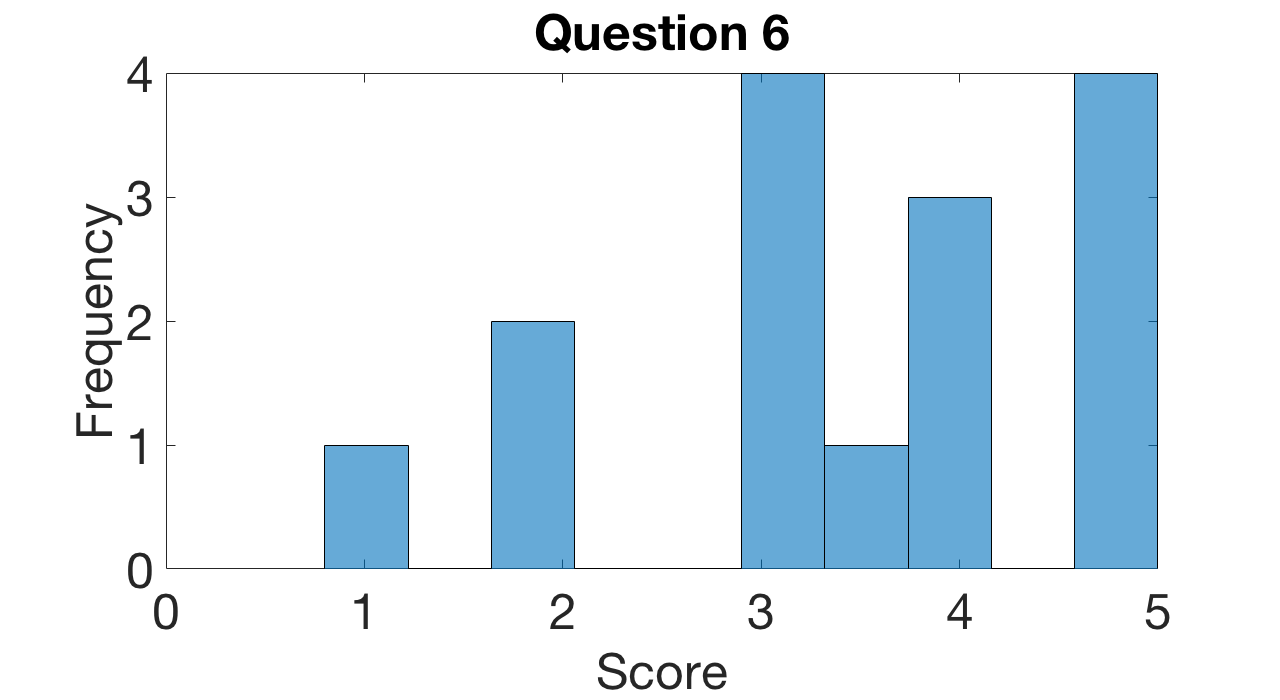
\includegraphics[width=\textwidth]{pics/q6}
				\caption{Question 6.}
				\label{fig:survey6}
		\end{subfigure}
	\caption{Histograms of survey results.}
	\label{fig:survey}
\end{figure}

\subsection{Comments}
There were a lot of comments about the UI. The first group of comments were about the colours. The use of colours for the risk was well received, with the ``traffic light'' system being something that everyone immediately recognised. However, constrast of the colour of the text with the colour of the background was questioned in certain cases. Additionally, a good point that was raised was the case of colour blindness, and how it would affect visibility of the messages.
\\\\
There was also the comment that the time it takes to get through to the user is too long. Those surveyed wondered if that would be a problem if speed was important. As for the feeling of listening to the messages, some felt that it was not nice to speak to a machine. Others thought that it was easy to confuse it for a wrong number! And upon encountering the goodbye message, some felt that it made them angry. Others felt demotivated to continue calling, and most agreed that an alternative contact method, such as a text or a Facebook message would be considered instead.

\end{document}
